\section{Fluid Flow}
\label{sec:NS_validation}


Two cases with no free surface are considered in Sections \ref{sec:validation_poiseille} and \ref{sec:validation_couette}. These are, in contrast to free surface tests, relatively unused validation cases for fluid flow in the hydraulics community. In recent years \ac{SPH} has matured rapidly as a method and current machines allow for large cases to be tested. Traditional dam-break flow, explored in \cite{Crespo-2007}, \cite{Violeau-2007} and \cite{Gomez-Gesteira-2010}, among others, were extensively validated, considering velocity of the wave front, free surface deformation and forces on static obstacles. For this reason, a less traditional approach is taken in Section \ref{sec:validation_dam_break}: experimental velocity fields from a downward gate set-up are compared with the numerical solution.

%%%%%%%%%%%%%%%%%%%%%%%%%%%%%%%%%%%%%%%%%%%%%%%%%%%%%%%%%%%%%%%%%
\subsection{Hagen-Poiseuille Flow}
\label{sec:validation_poiseille}

The first solution of the Navier-Stokes that will be explored is the Hagen-Poiseuille flow. The problem was first explored experimentally by Gotthilf Heinrich Ludwig Hagen in 1839 and Jean L\'{e}onard Marie Poiseuille in 1838, and published by Poiseuille in 1840 and 1846. The conditions are simple: the flow is laminar through a pipe of constant circular cross-section that is substantially longer than its diameter. The original experiments did not account for acceleration of fluid. For velocities and pipe diameters above a threshold, the fluid flow becomes turbulent, leading to larger pressure drops than calculated by the Hagen-Poiseuille equation.

Admitting conditions for a laminar Hagen-Poiseuille flow, the Navier-Stokes equations allow analytical solutions. A transient solution can be derived using Fourier series \citep{Drazin-2006} and \cite{Morris-1997} used the solution to test the laminar viscous term in Equation \eqref{eq:sph_morris_laminar}. Since the discretization of the momentum equation is not exactly the same, SPS terms are introduced and the solid boundary conditions are very different, the same exercise is reproduced here. Of special concern are the SPS terms, since the simple Smagorinsky model is known to introduce non-zero tensions in a laminar flow \citep{Batchelor-2000}. For a fluid initially at rest between stationary infinite plates at $y=0$ and $y=L$, with an applied body force $\ve{F}$, acting parallel to the axis of the channel, the series solution for the velocity $u$ along the channel cross-section is given by 

%
\begin{equation} \label{eq:Poiseuille_t}
	u(y,t)=-\frac{|\ve{F}|}{2\nu}y(y-L)-\sum^\infty_{n=0}\frac{4|\ve{F}|L^2}{\nu \pi^3 (2n+1)^3}\sin\left( \frac{\pi y}{L}(2n +1) \right)\exp\left( -\frac{(2n+1)^2\pi^2 \nu}{L^2}t \right)
\end{equation}
%
Employing $\nu=10^{-6}$ m$^2$s$^{-1}$, $L=10^{-3}$ m, $|\ve{F}|=10^{-4}$ ms$^{-2}$, the maximum velocity, taken from the first term of Equation \eqref{eq:Poiseuille_t} (or $t=\infty$) is $u_{max}=1.25\times10^{-5}$ ms$^{-1}$, resulting in $R_e=u_{max}L/\nu=1.25\times10^{-2}$. The 2D simulations were carried out with an initial particle spacing of $L/Dp=20$, $L/Dp=50$ and $L/Dp=150$ and a smoothing length defined as $h=\sqrt{2Dp^2}$, resulting in numerical solutions that can be compared with expression \eqref{eq:Poiseuille_t} at chosen time instants. The domain is $5\times10^{-3}$ m long and periodic conditions are applied in the longitudinal direction. Figure \ref{fig:Poiseuille} shows the numerical and time series solutions.

%
\begin{figure}[ht!]
	\centering
	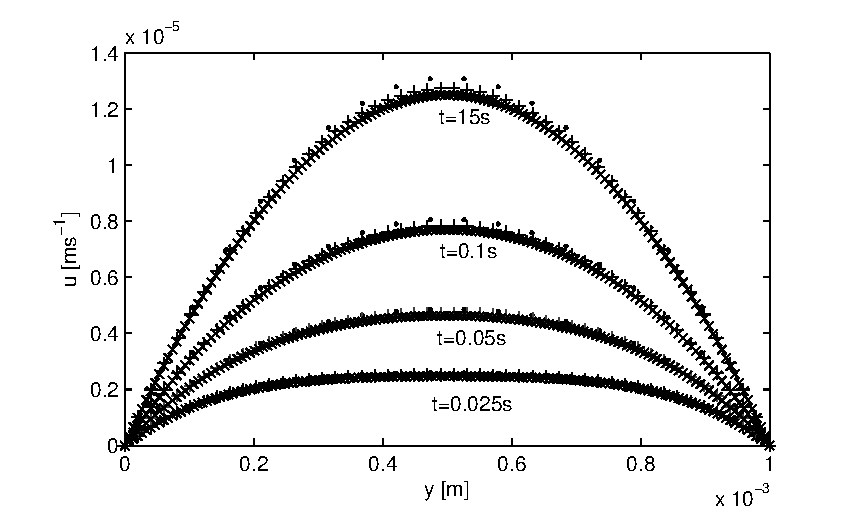
\includegraphics[width=0.70\linewidth]{Figures/5.Chapter/Poiseuille}
	\caption{Series solution (--) and SPH solution $L/Dp=20$ ($\cdot$), $L/Dp=50$ (+), $L/Dp=150$ ($\times$) for $R_e=1.25\times10^{-2}$, at several instants.}
	\label{fig:Poiseuille} 
\end{figure}
%
The results show that the transient nature of the flow is well captured at all resolutions and relative errors, although larger for the less resolved $L/Dp=20$ case, is limited to $5\%$, with the maximum of $0.1\%$ for the $L/Dp=150$ case. These results are compatible with the reported by \cite{Morris-1997}, indicating that the introduction of the \ac{SPS} terms does not appear to corrupt the laminar solution. Computing the \ac{RMSE} of the solution for $t=15$ s, we can obtain some insight into the convergence rate of the solution, as presented in Figure \ref{fig:HP_RMSE}.

%
\begin{figure}[ht!]
	\centering
	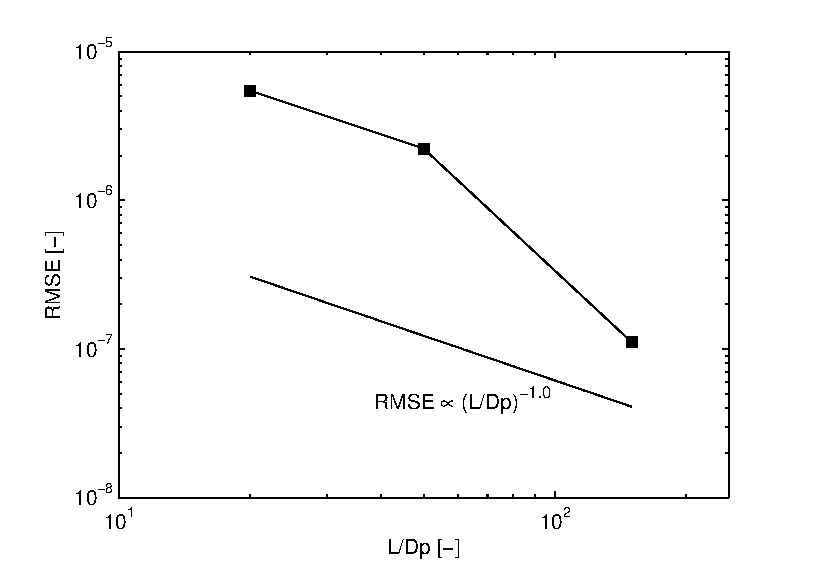
\includegraphics[width=0.70\linewidth]{Figures/5.Chapter/HP_RMSE}
	\caption{\ac{RMSE} with increasing resolution. Linear convergence slope for comparison.}
	\label{fig:HP_RMSE} 
\end{figure}
%
The convergence rate for increasing resolution seems to be supra linear in this case. A more complete convergence test would include changing the smoothing length $h$, as presented in \cite{Dehnen-2012}.

%%%%%%%%%%%%%%%%%%%%%%%%%%%%%%%%%%%%%%%%%%%%%%%%%%%%%%%%%%%%%%%%%
\subsection{Couette Flow}
\label{sec:validation_couette}

Couette flow is, similarly to the Poiseuille flow explored in the previous section, developed between two infinite plates. For the transient flow, the system is introduced at rest. For $t=0$ s, the upper plate starts to move parallel to the longitudinal direction, at a constant velocity $V_0$. This introduces a shear stress that promotes the flow. \cite{Drazin-2006} introduced the series solution amending the analytical solution

%
\begin{equation} \label{eq:Couette_t}
	u(y,t)=\frac{V_0}{L}y+\sum^\infty_{n=1}\frac{2V_0}{n\pi}(-1)^n\sin\left( \frac{n\pi}{L}y \right)\exp\left( -\frac{n^2\pi^2}{L^2}\nu t \right)
\end{equation}
%
The flow was modeled using $\nu=10^{-6}$ m$^2$s$^{-1}$, $L=10^{-3}$ m and $V_0=1.25\times10^{-5}$ ms$^{-1}$, with initial particle spacing of $L/Dp=20$, $L/Dp=50$ and $L/Dp=150$ and the same scheme constants as in last Section. The Reynolds number is also the same, $R_e=1.25\times10^{-2}$. The domain is $5\times10^{-3}$ m long and periodic conditions are applied in the longitudinal direction. Figure \ref{fig:Couette} shows the numerical and time series solutions.

%
\begin{figure}[ht!]
	\centering
	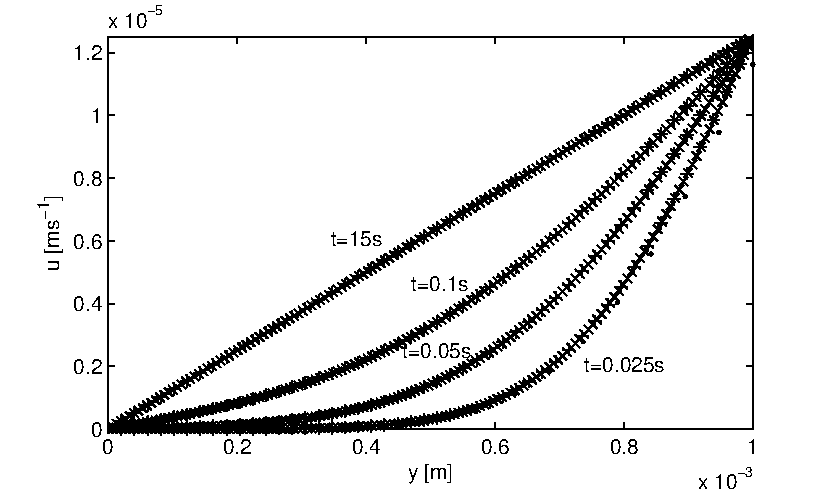
\includegraphics[width=0.70\linewidth]{Figures/5.Chapter/Couette}
	\caption{Series solution (--) and SPH solution $L/Dp=20$ ($\cdot$), $L/Dp=50$ (+), $L/Dp=150$ ($\times$) for $R_e=1.25\times10^{-2}$, at several instants.}
	\label{fig:Couette} 
\end{figure}
%
The numerical solution presents a good agreement. In the initial instant, the $L/Dp=20$ solution presents a deviation to the analytical velocity profile, with $5.8\%$ relative error in the vicinity of the mobile boundary. By the second instant however, the velocity profile is now coincident, with less than $0.7\%$ maximum error. Again, computing the \ac{RMSE} of the solution for $t=15$ s, in Figure \ref{fig:Ct_RMSE}, the convergence rate for the tested resolution range can be estimated.

%
\begin{figure}[ht!]
	\centering
	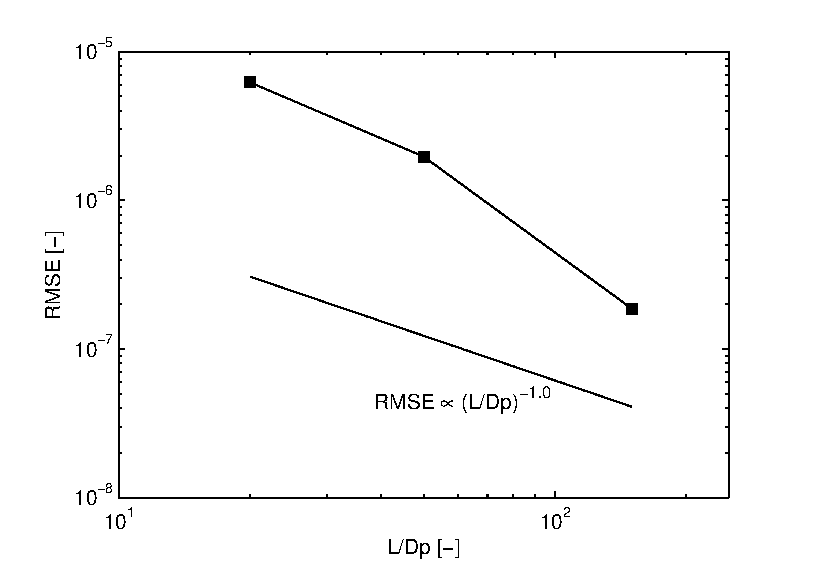
\includegraphics[width=0.70\linewidth]{Figures/5.Chapter/Ct_RMSE}
	\caption{\ac{RMSE} with increasing resolution. Linear convergence slope for comparison.}
	\label{fig:Ct_RMSE} 
\end{figure}
%
The convergence rate for the Couette case seems to be supra linear also, with the error distribution taking a similar form to the Haggen-Poiseuille case.



%%%%%%%%%%%%%%%%%%%%%%%%%%%%%%%%%%%%%%%%%%%%%%%%%%%%%%%%%%%%%%%%%
\subsection{Dam Break Flow}
\label{sec:validation_dam_break}

Advances in imaging techniques and processing power allow for the measure not only of the wave celerity and water level time series, but also the point-wise velocity field \citep{aleixo-al-2011, Oertel-2012}. This represents an interesting validation test for resolved models, since it allows to quantify not only global or average dynamics, but also local and time dependent quantities. The traditional dam break data used for validation \citep{Violeau-2007, Gomez-Gesteira-2010} relies on free surface deformation tracking and wave front velocity, but it is uncommon for experimental velocity profiles to be measured and numerical solutions to attempt comparisons.

An instantaneous dam break may be represented mathematically by an \ac{IVP}, simply as a discontinuity in the quantities. Due to the mathematical properties, most numerical studies are focused in this particular dam break. Different strategies can be found in the literature in order to experimentally simulate an instantaneous dam break, with the most used relying on the fast vertical displacement of a gate. This vertical displacement can be downward or upward as represented in Figure 1 b) and c) respectively. Upward moving gates are the traditional mechanism to study dam breaks. They present interesting qualities but introduce inevitable artificial sediment entrainment if the bed is covered with mobile sediment. Downward moving gates attempt to correct that effect, and have been used by \cite{Spinewine-2007} and \cite{Aleixo-2013}.

%
\begin{figure}[ht!]
	\centering
	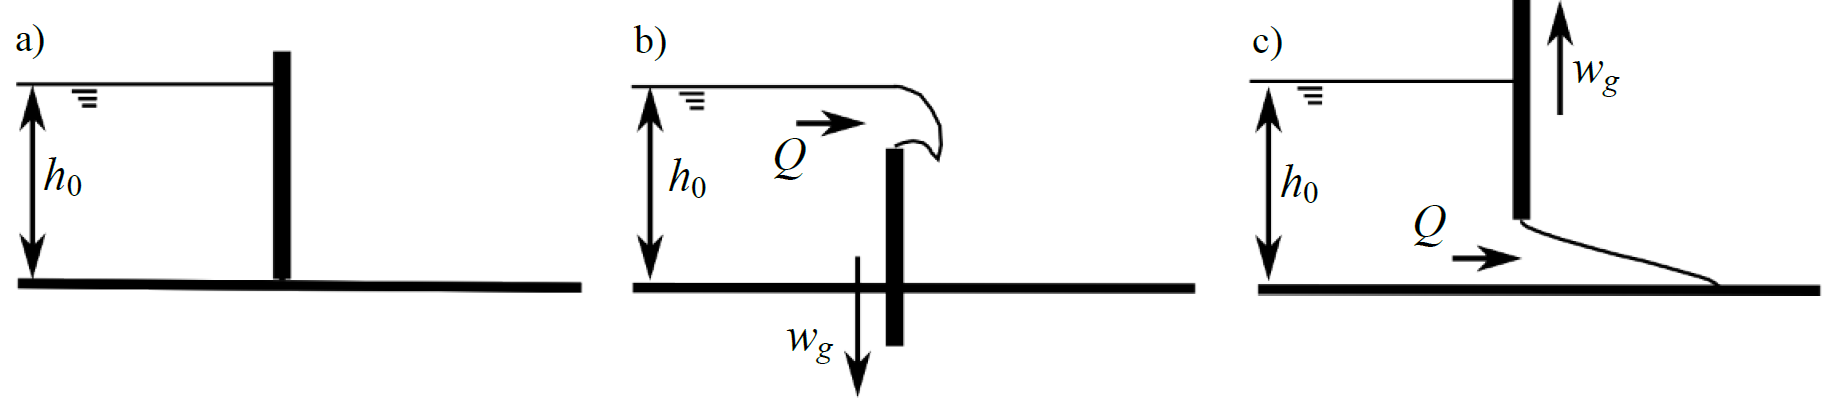
\includegraphics[width=0.90\linewidth]{Figures/5.Chapter/gate_comp}
	\caption{a) Scheme of a dam with initial height, $h_0$; b) downward moving gate; c) upward moving gate. $Q$ denotes the flow rate after the gate opening and $w_g$ the gate vertical velocity.}
	\label{fig:dam_squeme} 
\end{figure}
%

The measurements were carried in the dam-break channel of the Institute for Mechanics Materials and Civil Engineering, Universite Catholique de Louvain, Belgium. This channel is characterized by a width of 0.25 m, 0.50 m height and a 6 m length. Glass windows allow optical access to the flow. At half of its length a 0.0025 m thick aluminum gate was placed in order to simulate the dam-break flow. The gate separates the channel in two sections and is centered on the area of interest. This gate is connected to a pneumatic jack that drives the gate downward. The bottom of the reservoir section is made of impervious polished wood whereas the bottom of the test section is made of glass. 

To analyze flow a DALSA 1M150 fast camera was used. It has a maximum resolution of 1 Mpixel and an adjustable acquisition frequency of 150 Hz; in the present case however the acquisition frequency was set at 100 frames per second and an 8 mm lens was used. In order to measure the flow velocity the water of the reservoirs was seeded with High Density Polystyrene particles ($\rho/\rho_w = 0.94$), with a diameter of 2 mm. To improve the light reflection from the particles these were coated with a white paint. Combination of the particle density and the denser white coating made the resulting particles roughly neutrally buoyant \citep{aleixo-al-2011}. To track the particles motion a Vorono\"i-based particle tracking algorithm \citep{Capart-2002} was used.

\cite{Aleixo-2013} demonstrated that for a depth of $h_0=0.325$ m, the gate is removed in under 70 ms. This corresponds to an instantaneous removal, using the criteria from \cite{Lauber-1998}: $t_o(h_0=0.325)=\sqrt{2h_0/g}\approx0.26$ s. 

A 2D \ac{SPH} simulation was prepared with $Dp=0.001$ m, where the gate motion was imposed with the corresponding velocity. The smoothing length was $h=\sqrt{2Dp^2}$, the $C$ parameter from the stability region condition, Equation (\eqref{eq:sph_stability_region}), was set at $0.20$ and the kinematic viscosity is that of water at $20^{\circ}\;C$ temperature, $\nu = 10^{-6} \  \mathrm{m^2 s^{-1}}$. The velocity fields in Figures \ref{fig:comp_6} to \ref{fig:comp_17} represent the overlap of experimental and numerical data, interpolated to similar regular grids over the domain, over time. 

%
\begin{figure}[ht!]
	\centering
	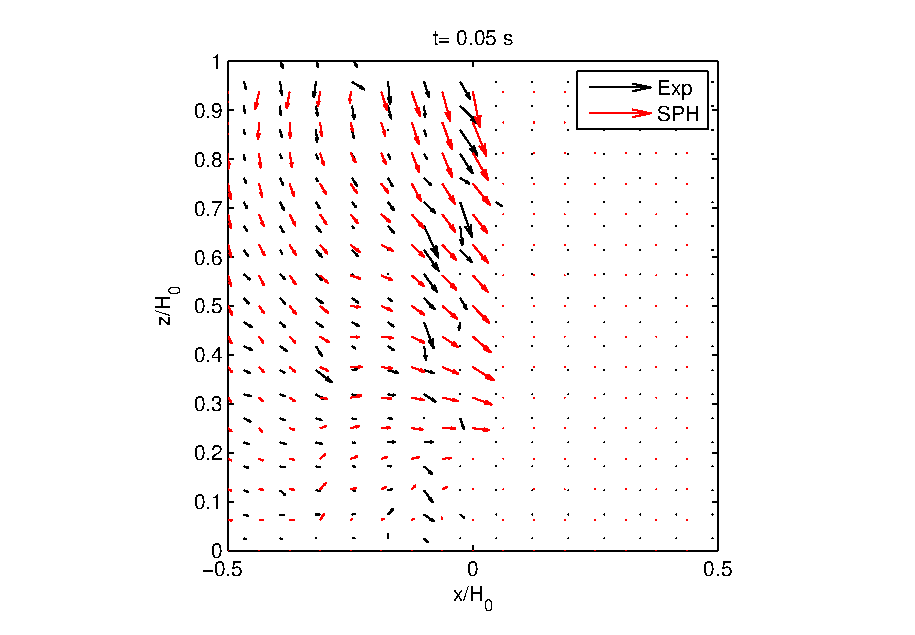
\includegraphics[width=0.70\linewidth]{Figures/5.Chapter/comp_6}
	\caption{Velocity fields, experimental and \ac{SPH} solution. $t=0.05$ s.}
	\label{fig:comp_6} 
\end{figure}
%

%
\begin{figure}[ht!]
	\centering
	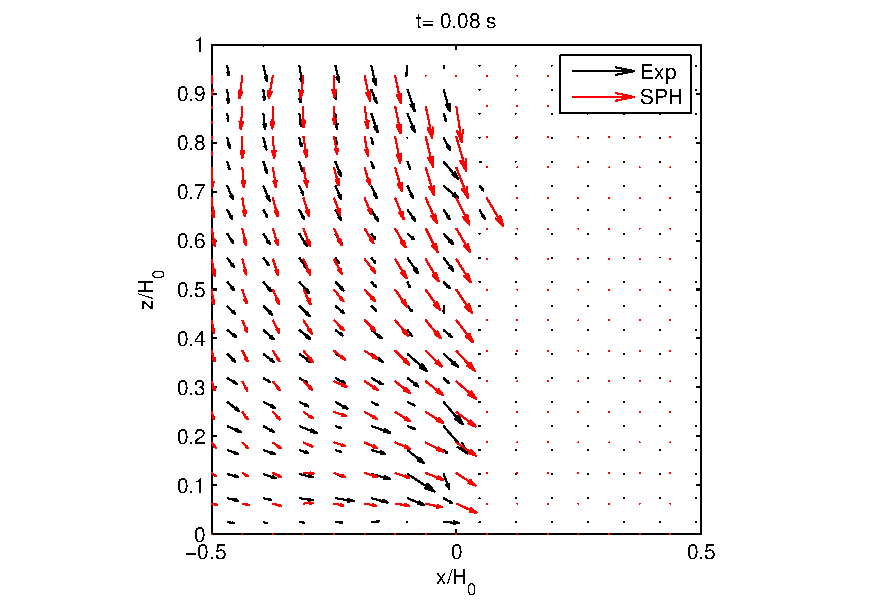
\includegraphics[width=0.70\linewidth]{Figures/5.Chapter/comp_9}
	\caption{Velocity fields, experimental and \ac{SPH} solution. $t=0.08$ s.}
	\label{fig:comp_9} 
\end{figure}
%

%
\begin{figure}[ht!]
	\centering
	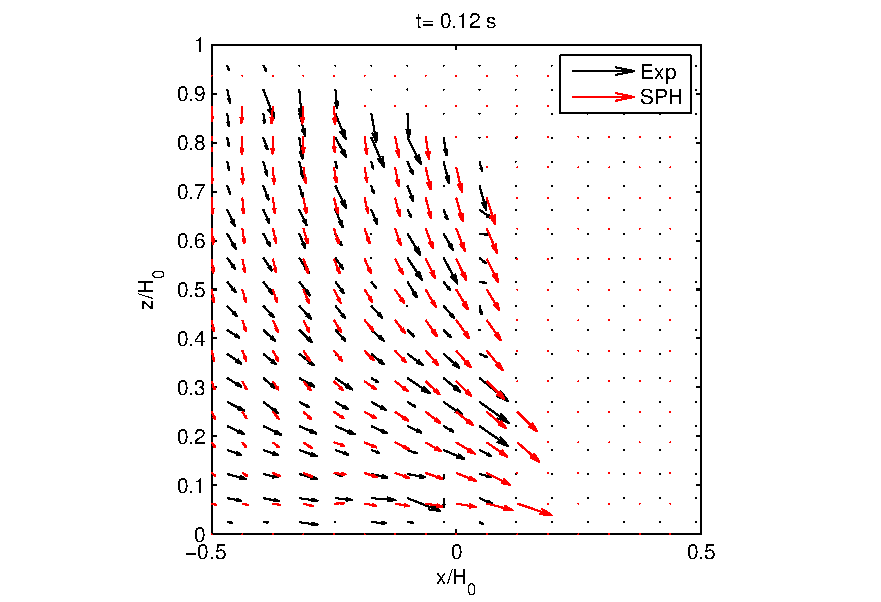
\includegraphics[width=0.70\linewidth]{Figures/5.Chapter/comp_13}
	\caption{Velocity fields, experimental and \ac{SPH} solution. $t=0.12$ s.}
	\label{fig:comp_13} 
\end{figure}
%

%
\begin{figure}[ht!]
	\centering
	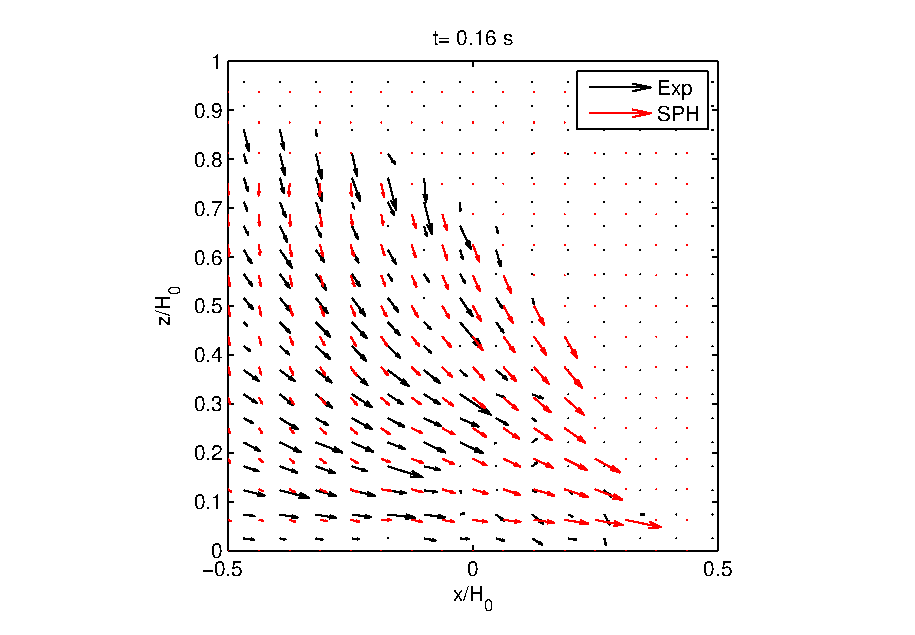
\includegraphics[width=0.70\linewidth]{Figures/5.Chapter/comp_17}
	\caption{Velocity fields, experimental and \ac{SPH} solution. $t=0.16$ s.}
	\label{fig:comp_17} 
\end{figure}
%

The velocity fields are quite similar in direction and the evolution on time of the \ac{SPH} solution seems consistent with the experimental data. To further quantify the differences, vertical profiles were derived, in Figures \ref{fig:Profiles_interps_8_8} to \ref{fig:Profiles_interps_8_20}, using a dimensionless velocity defined as 

%
\begin{equation} \label{eq:non_dim_vel}
	U=\frac{u_1}{\sqrt{gh_0}};\;\;\;\; W=\frac{u_2}{\sqrt{gh_0}},
\end{equation}
%
where $u_1$ and $u_2$ correspond to the horizontal and vertical velocity components, respectively.
%
\begin{figure}[H]
	\centering
	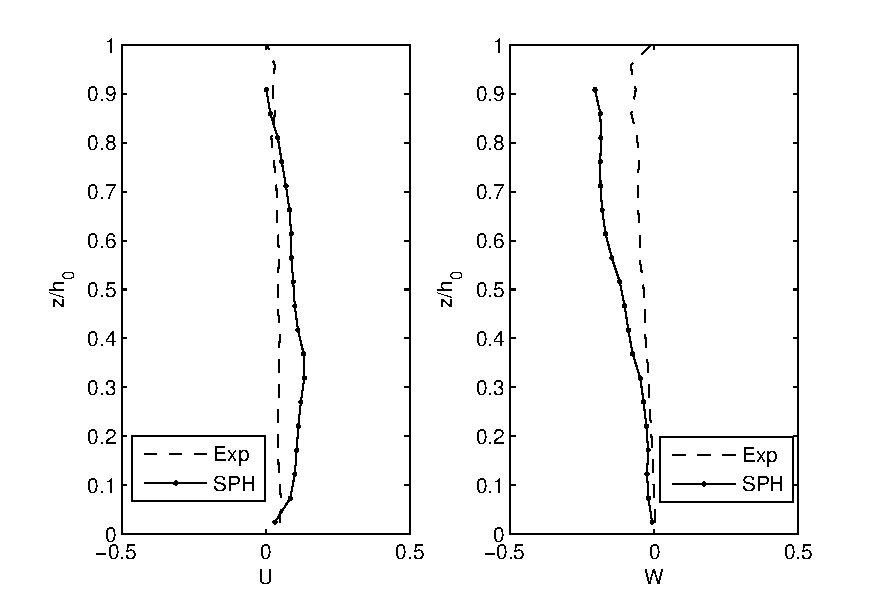
\includegraphics[width=0.65\linewidth]{Figures/5.Chapter/Profiles_interps_8_8}
	\caption{Velocity profiles, experimental and \ac{SPH} solution. $t=0.07$ s.}
	\label{fig:Profiles_interps_8_8} 
\end{figure}
%

%
\begin{figure}[H]
	\centering
	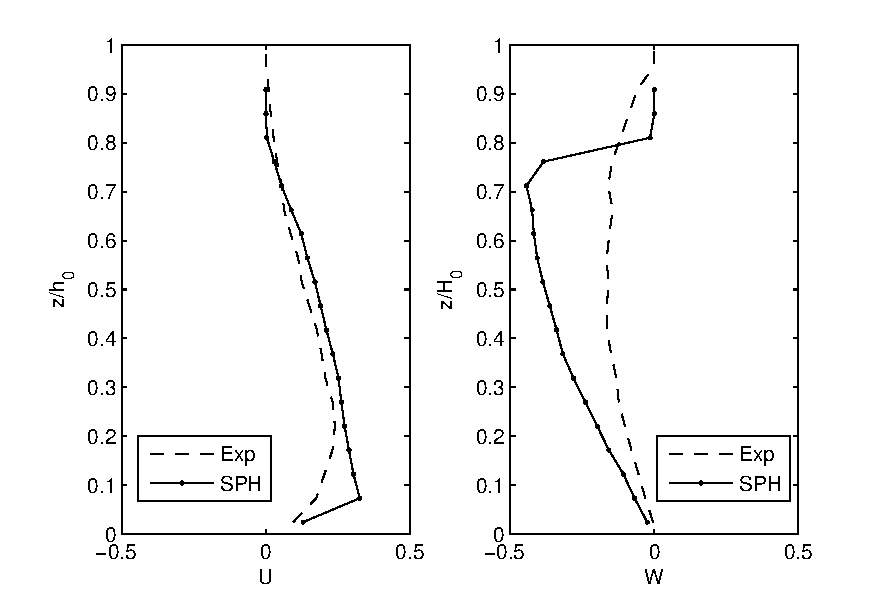
\includegraphics[width=0.65\linewidth]{Figures/5.Chapter/Profiles_interps_8_17}
	\caption{Velocity profiles, experimental and \ac{SPH} solution. $t=0.16$ s.}
	\label{fig:Profiles_interps_8_17} 
\end{figure}
%

%
\begin{figure}[H]
	\centering
	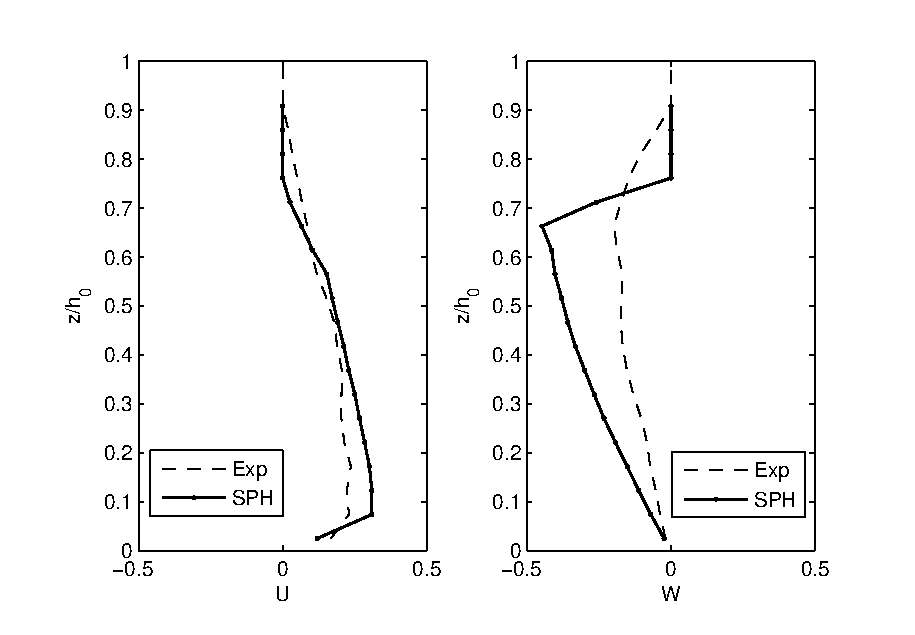
\includegraphics[width=0.65\linewidth]{Figures/5.Chapter/Profiles_interps_8_20}
	\caption{Velocity profiles, experimental and \ac{SPH} solution. $t=0.19$ s.}
	\label{fig:Profiles_interps_8_20} 
\end{figure}
%

The profiles show that the longitudinal velocity $u_1$ is well represented, showing the same tendencies as the experimental data. The vertical velocity $u_2$ seems to be larger on the numerical solution. The larger deviations may stem from experimental difficulties, as the tracer particles may suffer from a small upwards buoyant force. Experimental data was also interpolated and further smoothed to trace the profiles, as can be checked since the free surface does not seem to be well defined, also partly explaining the differences on the upper section of the flow, relative to the vertical velocity component, in Figures \ref{fig:Profiles_interps_8_17} and \ref{fig:Profiles_interps_8_20}. Note that the SPH profile is interpolated in points coinciding with the experimental measures, thus generating the visible gradient at the free surface area.

\clearpage
